\documentclass[11pt]{article}
\usepackage[margin=1in]{geometry}
\usepackage[T1]{fontenc}
\usepackage{lmodern,amsmath,amssymb,booktabs,graphicx,enumitem,array,xcolor}
\usepackage[most]{tcolorbox}
\usepackage[colorlinks,linkcolor=blue!50!black,urlcolor=blue!50!black]{hyperref}
\graphicspath{{../figs/}}
\setlength{\parskip}{5pt}\setlength{\parindent}{0pt}
\newcommand{\SP}{\ensuremath{\spadesuit}}\newcommand{\HE}{\ensuremath{\heartsuit}}
\newcommand{\DI}{\ensuremath{\diamondsuit}}\newcommand{\CL}{\ensuremath{\clubsuit}}
\newtcolorbox{example}[1][]{breakable,before upper={\setlength{\parskip}{5pt}},colback=blue!4,colframe=blue!45!black,title={Example. #1},fonttitle=\bfseries}
\newtcolorbox{intuition}{breakable,before upper={\setlength{\parskip}{5pt}},colback=green!5,colframe=green!40!black,title={Intuition},fonttitle=\bfseries}
\newtcolorbox{takeaway}{breakable,before upper={\setlength{\parskip}{5pt}},colback=orange!7,colframe=orange!70!black,title={What to remember},fonttitle=\bfseries}
\newcommand{\slide}[1]{\hfill{\small\itshape (slide #1)}}
\title{Study Guide\\[4pt]\large Range-Vectorized Discounted Regret Minimization for No-Limit Hold'em:\\ Complexity, Precision and Parallelism}
\author{}\date{}
\begin{document}
\maketitle
\vspace{-3em}
This guide explains everything in the talk from the ground up. It assumes calculus, basic linear algebra (vectors,
matrices, dot products) and basic probability. It does not assume any numerical analysis, game theory or poker. Each
section follows the same pattern: the idea in plain words, the formula, a worked example with small numbers, and what
to remember. Slide numbers refer to \texttt{tex/talk.pdf}.

\tableofcontents
\newpage

% ============================================================================
\section{The one-paragraph summary}
A poker \emph{solver} takes a situation in a poker hand and computes how two perfect players would play it. That
perfect play is called a \emph{Nash equilibrium}. Our solver finds it with one algorithm, \emph{discounted
counterfactual regret minimization} (DCFR). The algorithm repeats one simple step, called an iteration, a few hundred
times, and each iteration nudges the strategies closer to equilibrium.

The talk is about the \emph{numerical analysis} of this computation. Numerical analysis asks four questions about any
algorithm that computes with numbers:
\begin{enumerate}[nosep]
\item \textbf{Cost.} How much arithmetic does one step take, and how does that grow with the size of the problem?
\item \textbf{Accuracy.} How close is the answer, and how do we measure that?
\item \textbf{Precision.} Computers round numbers. Does the rounding hurt?
\item \textbf{Parallelism.} Can several processors share the work?
\end{enumerate}
Every technical slide answers one of these four questions for the poker solver.

% ============================================================================
\section{Poker in five minutes}\slide{4}
\subsection{The rules we need}
In Texas hold'em each player gets two private cards (a \emph{hand}). Five public cards (the \emph{board}) are dealt
in stages: three cards (the \emph{flop}), then one (the \emph{turn}), then one (the \emph{river}). There is a round of
betting after each stage. A player can \emph{check} (bet nothing), \emph{bet}, \emph{call} (match a bet),
\emph{raise} (bet more) or \emph{fold} (give up). If nobody folds, the hands are compared at the \emph{showdown} and
the best five-card poker hand wins the \emph{pot}, the money in the middle. The \emph{stack} is the money a player has
left to bet.

Two players remain in our spots. The one who acts first is \emph{out of position} (OOP) and the other is \emph{in
position} (IP). In the running example the OOP player is the \emph{big blind} and the IP player is the \emph{button}.

\subsection{Ranges}
You never know the opponent's hand, but you know which hands are plausible given how the hand was played. A
\textbf{range} is a list of possible hands with a weight between 0 and 1 for each. Mathematically a range is a
vector, one number per hand. This is the key modelling idea: the solver never works with one hand, it works with a
whole vector of hands at once.

\begin{example}[Counting hands]
There are $\binom{52}{2} = 1326$ two-card hands. Once three flop cards are on the board, a hand must avoid them, which
leaves $\binom{49}{2} = 1176$ hands. On the turn there are $\binom{48}{2}=1128$ and on the river
$\binom{47}{2}=1081$. These are the three numbers on slide 4. In the running example the flop is
K\SP\,7\DI\,2\CL; the big blind's range has 488 hands with positive weight and the button's has 460.
\end{example}

\subsection{The subgame and the unknowns}
A \emph{subgame} (or \emph{spot}) is specified by: the board, the pot, the stack, one range per player, and a
\emph{bet tree}, the list of bet sizes we allow (for instance ``bet 33\% of the pot or check''). Real poker allows any
bet size; a solver restricts to a few, which makes the game finite.

The \textbf{unknowns} are: for every decision point in the tree and every hand, the probability of each action.
For example ``at the first decision, with A\SP K\SP, bet 70\% of the time and check 30\%.''

\begin{example}[How big is it?]
The flop tree with one bet size per street has 56{,}842 decision points. With about 470 hands and 2 to 3 actions each,
that is about 54 million unknown numbers. Why so many decision points when the betting is simple? After the flop
betting, any of 49 turn cards can come, and after the turn betting any of 48 river cards. Each card creates its own
copy of the rest of the tree: roughly $49\times48\approx 2350$ copies of the river betting.
\end{example}

\begin{takeaway}
A range is a vector of weights over hands. A spot is board, pot, stack, two ranges and a bet tree. The solution is a
table of action probabilities, and on the flop it has tens of millions of entries.
\end{takeaway}

% ============================================================================
\section{Games, equilibrium and exploitability}\slide{5}
\subsection{Zero-sum games and mixed strategies}
A game is \emph{zero-sum} when one player's gain is the other's loss. A \emph{mixed strategy} chooses actions at
random with chosen probabilities. Mixing is necessary: if you always bet your strong hands and never bluff, the
opponent simply folds whenever you bet.

\begin{example}[Rock--paper--scissors as a matrix]
Write the row player's winnings as a matrix, rows and columns in the order rock, paper, scissors:
\[ A=\begin{pmatrix} 0&-1&1\\ 1&0&-1\\ -1&1&0\end{pmatrix}. \]
If the row player mixes with probabilities $x$ and the column player with $y$, the average winnings are $x^\top A y$.
With $x=(\tfrac12,\tfrac12,0)$ and $y=(1,0,0)$ (always rock): $Ay = (0,1,-1)^\top$ and
$x^\top A y = \tfrac12\cdot0+\tfrac12\cdot1 = 0.5$. The expression $x^\top A y$ is linear in $x$ and linear in $y$;
that is what ``bilinear'' on the slide means.
\end{example}

\subsection{Nash equilibrium and the minimax theorem}
A pair of strategies is a \textbf{Nash equilibrium} if neither player can gain by changing strategy alone. Von
Neumann's minimax theorem says that in a zero-sum game such a pair always exists and that the game has a single
\emph{value} $v^\ast$: the first player can guarantee at least $v^\ast$, and the second can hold the first to at most
$v^\ast$,
\[ \max_x\min_y x^\top A y=\min_y\max_x x^\top A y=v^\ast. \]
In rock--paper--scissors the equilibrium is $(\tfrac13,\tfrac13,\tfrac13)$ for both and the value is 0.

\begin{example}[A one-street poker game you can solve by hand]
The pot is 1. The bettor holds either the best hand (the ``nuts'') or a hopeless hand (``air''), each half of the time.
The caller holds a medium hand that beats air and loses to the nuts. The bettor may bet 1 or check; after a bet the
caller may call or fold.

\emph{Bettor.} Always bet the nuts. Bluff with air just often enough that the caller does not care whether she calls.
The caller risks 1 to win 2 (the pot plus the bet), so she is indifferent when $2\cdot\Pr(\text{air})=1\cdot
\Pr(\text{nuts})$ among the betting hands: one bluff for every two value bets. So bluff with air half of the time.

\emph{Caller.} Call just often enough that the bettor does not care whether he bluffs. A bluff wins 1 if she folds and
loses 1 if she calls: $(1-c)-c=0$, so call with probability $c=\tfrac12$.

That pair is the equilibrium. The bettor's value: with the nuts he wins $1+\tfrac12\cdot 1=1.5$, with air he wins 0
on average, so $\tfrac12\cdot1.5=0.75$ of the pot.
\end{example}

\subsection{Exploitability: how we measure error}
A solver never reaches the exact equilibrium; it gets close. We need a number that says how close. The
\textbf{exploitability} of a pair of strategies is the average amount the two players could gain if each switched to
the best possible reply (the \emph{best response}) against the other:
\[ \mathrm{expl}(x,y)=\tfrac12\Big(\underbrace{\max_{x'}x'^\top Ay}_{\text{best reply to }y}-
\underbrace{\min_{y'}x^\top Ay'}_{\text{best reply to }x}\Big)\ \ge 0. \]
It is zero exactly at an equilibrium. We report it as a percentage of the pot. Commercial solvers stop at 0.1\% to
0.5\%; our default target is 0.3\%.

\begin{example}[Exploitability in the toy game]
Suppose the bettor plays the equilibrium but the caller always folds. The bettor's best reply is to bet every hand and
win the pot every time: value 1 instead of 0.75, a gain of 0.25. The caller cannot gain anything against the
equilibrium bettor (she is indifferent). Exploitability $=\tfrac12(0.25+0)=0.125$, that is 12.5\% of the pot. A
solver would call this strategy pair very inaccurate.
\end{example}

\begin{intuition}
Exploitability plays the role that ``error'' plays elsewhere in numerical analysis, with one advantage: it can be
computed without knowing the true answer. You only need to compute two best responses. In optimization language it is
the \emph{duality gap}.
\end{intuition}

\textbf{Rake.} If the casino takes a fee from the pot (rake), the game is no longer zero-sum and the theorems do not
apply. The solver still runs and still reports how much each player could gain by deviating.

\begin{takeaway}
Equilibrium = nobody can improve alone. Exploitability = how much the players could still gain; it is the solver's
error measure, it is computable, and 0.3\% of the pot is ``solved'' in practice.
\end{takeaway}

% ============================================================================
\section{Regret matching and CFR}\slide{6}
\subsection{Regret}
After a round of a game, ask about each action: ``how much better would I have done if I had played this action
instead of what I did?'' That difference is the \textbf{regret} of the action for that round. Add the regrets over
all rounds to get the \emph{cumulative regret} $R(a)$.

\textbf{Regret matching} is the rule: next round, play each action with probability proportional to its positive
cumulative regret,
\[ \sigma(a)=\frac{\max(R(a),0)}{\sum_b\max(R(b),0)}, \]
and play uniformly if no regret is positive. Actions you wish you had played more get played more.

\begin{example}[Two rounds of rock--paper--scissors by hand]
\textbf{Round 1.} You start uniform, $(\tfrac13,\tfrac13,\tfrac13)$. The opponent plays rock. The actions would have
earned: rock 0, paper $+1$, scissors $-1$. Your average was 0. Regrets: $(0,\,1,\,-1)$. Positive parts: $(0,1,0)$. Next
strategy: always paper.

\textbf{Round 2.} You play paper, the opponent plays scissors. The actions would have earned: rock $+1$, paper $-1$,
scissors 0. You earned $-1$. Regrets this round: $(2,\,0,\,1)$. Cumulative: $(2,\,1,\,0)$. Next strategy:
$(\tfrac23,\tfrac13,0)$.
\end{example}

The remarkable fact (Hart and Mas-Colell, 2000): if both players use regret matching, their \emph{average}
strategies over all rounds converge to an equilibrium. Note the word average. The strategy of the latest round can
keep swinging; the running average settles down.

\subsection{From one decision to a whole tree: counterfactual regret}
Poker has many decision points. CFR (Zinkevich and coauthors, 2007) runs a separate regret matching at every decision
point for every hand. The mathematical name for ``a decision point as seen by a player holding a specific hand'' is an
\emph{information set}.

The payoff fed into each local regret matching is the \textbf{counterfactual value}: the value of an action, weighted
by the probability that the \emph{opponent and the cards} lead to this point. That probability is called the
opponent's \emph{reach}.

\begin{example}[A counterfactual value]
You hold the medium hand of the toy game and face a bet of 1 into a pot of 1. The opponent's hands are nuts and air,
each with prior weight $\tfrac12$. He bets the nuts always and air half the time, so his reach at this point is
$\tfrac12\cdot1=0.5$ for the nuts and $\tfrac12\cdot\tfrac12=0.25$ for air. Calling loses 1 against the nuts and wins
2 against air:
\[ v(\text{call}) = 0.5\cdot(-1)+0.25\cdot(+2)=0,\qquad v(\text{fold})=0. \]
Both actions have the same value, so the regrets do not move: this is the equilibrium. If he bluffed more, the reach
of air would be larger, calling would have positive regret, and you would call more next iteration.
\end{example}

\subsection{The theorem and why its bound is useless in practice}
The theorem on slide 6 says the exploitability of the average strategies after $T$ iterations is at most
\[ \frac{\Delta\,|\mathcal I|\,\sqrt{|A|}}{\sqrt T}, \]
where $\Delta$ is the largest possible swing in payoff, $|\mathcal I|$ the number of information sets and $|A|$ the
number of actions. Two messages:
\begin{itemize}[nosep]
\item It goes to zero as $T$ grows, so CFR \emph{does} converge. To halve the bound you need four times the
iterations (that is what $1/\sqrt T$ means).
\item The constant is enormous. On the flop spot $\Delta\approx195$ chips, $|\mathcal I|\approx 2.7\times10^7$,
$\sqrt{3}\approx1.7$. At $T=10{,}000$ the bound is about $9\times10^{7}$ chips for a pot of 5.5 chips. The bound is
true but tells us nothing; the slide calls it \emph{vacuous}.
\end{itemize}
In practice the method is far faster than the bound, which is why the talk \emph{measures} convergence instead of
relying on the theorem (Section~\ref{sec:conv}).

\begin{takeaway}
CFR = regret matching at every decision point for every hand, using values weighted by the opponent's reach. The
average strategy converges. The proven rate $1/\sqrt{T}$ is a guarantee, not a prediction.
\end{takeaway}

% ============================================================================
\section{Discounted CFR}\slide{7}
\subsection{The idea}
The first iterations of CFR are bad: the strategies are nearly random, and so are the regrets they produce. Plain CFR
keeps these early regrets forever. \textbf{DCFR} (Brown and Sandholm, 2019) multiplies the old sums by a number
slightly less than 1 before adding the new terms, so old information fades:
\begin{align*}
\text{positive regrets:}&\quad R\leftarrow R\cdot\frac{t^{1.5}}{t^{1.5}+1}+\text{new regret},\\
\text{negative regrets:}&\quad R\leftarrow R\cdot\tfrac12+\text{new regret},\\
\text{strategy sums:}&\quad S\leftarrow S\cdot\Big(\frac{t}{t+1}\Big)^{2}+\text{reach}\times\text{current strategy}.
\end{align*}
These are the formulas of slide 7 with $(\alpha,\beta,\gamma)=(1.5,\,0,\,2)$. The strategy sum $S$ is what the
average strategy is computed from.

\begin{example}[The discount on the rock--paper--scissors numbers]
After round 1 the regrets were $(0,1,-1)$. At $t=2$ the positive factor is $2^{1.5}/(2^{1.5}+1)=2.83/3.83=0.74$ and
the negative factor is $\tfrac12$. Discounted: $(0,\,0.74,\,-0.5)$. Add the round-2 regrets $(2,0,1)$: $(2,\,0.74,\,
0.5)$. New strategy: $(0.62,\,0.23,\,0.15)$, compared with $(0.67,0.33,0)$ for plain CFR. The early ``paper is great''
signal has faded a little, and the action that looked bad (scissors) recovers sooner because its negative regret was
halved.
\end{example}

\begin{example}[How much the average forgets]
With $\gamma=2$, iteration $t$ gets weight proportional to $t^2$ in the average. After 10 iterations the weights are
$1,4,9,\dots,100$, which sum to 385. Iteration 1 counts for $1/385=0.26\%$; with a plain average it would count for
10\%. Iteration 10 counts for 26\%.
\end{example}

\textbf{One family, three methods.} Setting the exponents to infinity turns the discount off. Plain CFR is
$\alpha=\beta=\infty,\gamma=0$. CFR$^+$, an earlier improvement, is $\alpha=\infty$, $\beta=-\infty$ (negative regrets
reset to zero), $\gamma=1$. The same code runs all three, which makes the comparison in Section~\ref{sec:conv} fair.

\textbf{Alternating updates.} Instead of updating both players from the same old strategies, we update player 1,
then update player 2 against player 1's \emph{new} strategy. If you have seen iterative methods for linear systems,
this is Gauss--Seidel versus Jacobi: use fresh information as soon as you have it. The theorem on the slide is proved
for simultaneous updates; alternation is standard practice.

\subsection{A bug story worth telling: exactness}
If the opponent never reaches some part of the tree (reach zero), every value there is zero, so it is tempting to skip
that part entirely. An early version did. But skipping also skipped the \emph{discounting} and the strategy-sum
updates in that part, so the code was no longer running DCFR. On a small flop game the exploitability after 1000
iterations was 0.64 chips instead of 0.0025: 250 times worse.

The fix: still visit those subtrees to apply discounts and strategy sums, and skip only the leaf evaluations (which
really are zero). A test now checks that the result agrees \emph{bit for bit} with a version that never skips.

\begin{takeaway}
DCFR = CFR with fading memory. A shortcut is only valid if it leaves the algorithm's numbers exactly unchanged, and
that should be tested.
\end{takeaway}

% ============================================================================
\section{Organizing one iteration: vectors on the public tree}\slide{8}
\subsection{The public tree}
The \textbf{public tree} contains only what both players can see: bets and board cards. Private hands are not in the
tree. Instead, every node carries \emph{vectors} indexed by hands.

One iteration consists of one \emph{traversal} per player. A traversal for player $p$ walks the tree and
\begin{itemize}[nosep]
\item carries \emph{down} the opponent's reach vector (how likely each opponent hand is to arrive here),
\item brings back \emph{up} a value vector (how much each of $p$'s hands is worth here).
\end{itemize}
What happens at each kind of node:
\begin{description}[nosep,leftmargin=1.5em]
\item[Opponent's decision.] For each action, multiply the reach entrywise by the probability that each hand takes
that action, go down, and add up the values that come back.
\item[Own decision.] Go down every action, combine the returned values weighted by the current strategy, and update
the regrets $R$ and strategy sums $S$.
\item[Chance node] (a card is dealt). Average over the possible cards.
\item[Leaf] (fold or showdown). Compute the payoff of each own hand against the opponent's reach.
\end{description}

\begin{example}[Reach vectors going down]
The opponent has three hands (AA, KQ, 72) with reach $(1,\,1,\,1)$ at a node where he can bet or check. His current
strategy is to bet with probabilities $(1,\,0.5,\,0.3)$. The reach passed to the ``bet'' child is the entrywise
product $(1,\,0.5,\,0.3)$ and to the ``check'' child $(0,\,0.5,\,0.7)$. If you now see a bet, the vector says: AA is
certain to play this way, 72 rarely does.
\end{example}

\subsection{Why this matters for cost}
At a decision node with $n$ hands and $|A|$ actions, the work is about $n\times|A|$ multiplications and additions:
we say it costs $O(n|A|)$. (``$O(\cdot)$'' means ``proportional to, for large inputs''.)

\begin{intuition}
A naive program would walk the tree once for every pair of hands: $488\times460\approx224{,}000$ walks per
iteration. The vector version walks it twice per iteration (once per player) and does a short loop over hands at each
node. Computers are very fast at such loops over numbers stored next to each other in memory. ``Action-major storage''
on the slide means the numbers are laid out so that the inner loop runs over hands, in order.
\end{intuition}

\textbf{Link to the matrix picture.} In Section 3 the payoff was $x^\top A y$. An iteration needs the products $Ay$
and $A^\top x$. The traversal computes exactly these products without ever writing the matrix $A$ down, which would be
impossible: $A$ would have a $500\times500$ block for every one of about seventy thousand leaves.

\begin{takeaway}
One iteration = two walks of the public tree with vectors over hands. Cost per decision node is proportional to
(hands) $\times$ (actions).
\end{takeaway}

% ============================================================================
\section{Chance nodes: the factor $1/K$}\slide{9}
When a card is dealt, the value of a hand is the average of its values over the possible cards. The question is:
average over how many cards?

Fix one hand for each player. Then $3$ (or 4) board cards and $2+2$ private cards are known, and the next card is
equally likely to be any of the others:
\[ K = 52-|\text{board}|-4 = 48-|\text{board}|,\qquad K=45\text{ on the flop},\quad K=44\text{ on the turn}. \]
So each card gets weight $1/K$. The formula on the slide,
\[ v(h)=\frac1K\sum_{c\notin\text{board}}\mathbf 1[c\notin h]\;v^{(c)}(h), \]
reads: add up the values over cards $c$ that are not in my hand $h$ (the symbol $\mathbf 1[\cdot]$ is 1 when the
condition holds and 0 otherwise), and divide by $K$. The opponent's hands that contain $c$ are removed by setting
their reach to zero for that card.

\begin{example}[Why not $1/49$?]
On the flop there are 49 cards that are not on the board, so $1/49$ looks natural. But 4 of them are in the two
players' hands. For any specific pair of hands only 45 cards can come, so with weight $1/49$ the probabilities would
add to $45/49$, not 1, and every value would be about 8\% too small.
\end{example}

\begin{intuition}
The nice surprise is that $K$ is the same number for every pair of hands. So the chance node is a plain sum times a
constant. No bookkeeping per hand is needed.
\end{intuition}

% ============================================================================
\section{Leaves in linear time}\label{sec:leaves}\slide{10--11}
A leaf is where the hand ends. This is where most naive solvers lose their time, and where the main trick of the
talk lives.

\subsection{The problem: card removal}
Two players cannot hold the same card. If I hold A\SP K\SP, the opponent cannot hold A\SP Q\HE. So at a leaf, the
value of my hand must only count the opponent hands that share no card with mine. Poker players call this
\emph{card removal} or \emph{blockers}.

The direct way: for each of my $n$ hands, loop over all $n$ opponent hands and skip the clashing ones. That is $n^2$
operations: about a million for $n=1000$, at every one of tens of thousands of leaves.

\subsection{Fold leaves: inclusion--exclusion}
At a fold leaf the payoff is the same against every opponent hand, so all I need is the total opponent weight that
does not clash with my hand $h=(h_1,h_2)$:
\[ m(h)=\tau-s_{h_1}-s_{h_2}+r_{\bar h}. \]
Here $\tau$ is the total opponent weight, $s_c$ is the total weight of opponent hands containing card $c$, and
$r_{\bar h}$ is the weight of the opponent hand identical to mine.

Why it works: start with everything ($\tau$). Remove the hands containing my first card, then those containing my
second card. A hand containing \emph{both} my cards (only the identical hand) has now been removed twice, so add it
back once. This is the inclusion--exclusion principle.

\begin{example}[Fold leaf by hand]
I hold A\SP K\SP. The opponent's range and reach:
\begin{center}\begin{tabular}{lccccc}
\toprule hand & A\SP Q\HE & K\SP K\HE & A\HE K\HE & Q\DI Q\CL & 7\DI 6\DI\\
\midrule reach & 0.5 & 1 & 1 & 1 & 0.5\\ \bottomrule
\end{tabular}\end{center}
Direct count: the hands that do not clash with mine are A\HE K\HE, Q\DI Q\CL{} and 7\DI 6\DI, total $1+1+0.5=2.5$.

Formula: $\tau=4$; hands with A\SP: $s_{A\spadesuit}=0.5$; hands with K\SP: $s_{K\spadesuit}=1$; identical hand: 0.
So $m=4-0.5-1+0=2.5$. \checkmark

Now add A\SP K\SP{} itself to his range with reach 0.3: $\tau=4.3$, $s_{A\spadesuit}=0.8$, $s_{K\spadesuit}=1.3$,
$m=4.3-0.8-1.3+0.3=2.5$. \checkmark{} The identical hand was subtracted twice and added back once.
\end{example}

The cost: one pass over the opponent's hands computes $\tau$ and the 52 card sums; one pass over my hands applies the
formula. That is proportional to $n$, not $n^2$.

\textbf{The matrix view} (bottom of slide 10). The ``who is compatible with whom'' table is the all-ones matrix,
minus a correction for each of the 52 cards, plus a fix for identical hands. A matrix that is ``simple plus a few
corrections'' can be multiplied by a vector quickly. This is a common theme in numerical linear algebra:
\emph{exploit structure instead of storing the matrix}.

\subsection{Showdown leaves: sort, then sweep}
At a showdown my hand wins against weaker hands, loses to stronger ones and ties with equal ones. If the opponent's
hands are \emph{sorted by strength}, then ``total weight of hands weaker than mine'' is a running total (a
\emph{prefix sum}). Walk up both sorted lists once, keeping a running total, and every hand gets its answer.

The formula on slide 11:
\[ v(h)=\ell\,m(h)+(w-\ell)\,L(h)+(\theta-\ell)\big(L^{=}(h)-L(h)\big), \]
with $w,\ell,\theta$ the payoffs for a win, loss and tie, $L(h)$ the compatible weight strictly weaker than $h$,
$L^{=}(h)$ the weight weaker or equal, and $m(h)$ the total compatible weight from the fold formula. Read it as:
``assume I lose to everyone ($\ell\,m$), then correct for the hands I beat and the hands I tie.''

\begin{example}[Showdown sweep by hand, ignoring card removal]
The pot gives $w=+5$ for a win, $\ell=-5$ for a loss, $\theta=0$ for a tie. The opponent's hands, sorted:
\begin{center}\begin{tabular}{lcccc}
\toprule strength & 1 & 3 & 3 & 6\\ \midrule reach & 0.5 & 1 & 0.5 & 1\\
running total & 0.5 & 1.5 & 2.0 & 3.0\\ \bottomrule
\end{tabular}\end{center}
My hand has strength 3. Weaker weight $L=0.5$. Weaker-or-equal $L^{=}=2.0$. Total $m=3.0$.
\[ v=-5\cdot3+10\cdot0.5+5\cdot(2.0-0.5)=-15+5+7.5=-2.5. \]
Check directly: I beat 0.5 ($+2.5$), tie 1.5 ($0$), lose to 1.0 ($-5$): total $-2.5$. \checkmark
\end{example}

Card removal is handled inside the sweep by the same trick as for folds: keep 52 running card sums alongside the
running total and subtract the two that belong to my cards. The sorting is done once per board and reused in every
iteration.

\subsection{What the measurements say}
\begin{center}\begin{tabular}{rrrr}
\toprule
$n$ & fold & showdown & direct \\ \midrule
50 & 0.5 & 1.2 & 10 \\
100 & 0.5 & 2.2 & 46 \\
200 & 0.9 & 3.0 & 276 \\
400 & 2.3 & 5.5 & 1193 \\
700 & 3.3 & 9.2 & 3773 \\
1081 & 5.9 & 13.7 & 4272 \\
\bottomrule
\end{tabular}
\end{center}
Times in microseconds for one leaf with $n$ hands. Doubling $n$ roughly doubles the fold and showdown times (linear)
but roughly quadruples the direct time (quadratic). At $n=1081$ the sweep is about 300 times faster, and the two
methods agree to 12 digits. One flop traversal evaluates about 42{,}000 showdown leaves, so this is the difference
between seconds and many minutes per iteration.

\begin{takeaway}
Card removal looks like an $n^2$ problem. Inclusion--exclusion (folds) and sort-then-running-total (showdowns) make
every leaf cost proportional to $n$. Check a fast method against the slow obvious one.
\end{takeaway}

% ============================================================================
\section{How long does an iteration take? A cost model}\slide{12}
\subsection{What a cost model is}
A cost model is a formula that explains running time from counts of work. Ours has two counts:
\[ T\approx a\,W_{\text{dec}}+b\,W_{\text{show}}. \]
$W_{\text{dec}}$ is the number of (hand, action) entries over all decision nodes: the size of the regret table.
$W_{\text{show}}$ is the number of hands summed over the showdown leaves that were evaluated. The constants $a$ and
$b$ are ``nanoseconds per unit of work'' and are found by \emph{least squares}: choose $a,b$ so the formula matches
the measured times of many runs as well as possible. (A nanosecond, ns, is a billionth of a second.)

The fit gives $a=30$ ns and $b=17$ ns from 252 timed iterations on 8 trees.

\begin{example}[Checking the model on the flop tree]
The one-size flop tree stores 431 MB at 8 bytes per entry, so $W_{\text{dec}}\approx 54$ million.
Decision part: $30\text{ ns}\times54\times10^6\approx1.6$ s. The showdowns add about 0.66 s (29\% of the total).
Sum: about 2.3 s. Measured: 2.28 s per iteration.
\end{example}

\subsection{How do we know the model is not just memorizing?}
Fit the constants on seven trees, then predict the eighth, which the fit has never seen. Repeat for each tree. This
is \emph{hold-out} (or leave-one-out) validation. The errors are 7\% and 10\% on the two big flop trees, and up to
30\% on tiny trees, where an iteration takes a few milliseconds and timing noise is large.
\begin{center}\begin{tabular}{lrrr}
\toprule
tree & decisions & measured & model \\ \midrule
turn, 1 size & 580 & 21 & 20 \\
turn, raises and all-in & 2,216 & 93 & 92 \\
flop, checked down later & 8 & 292 & 299 \\
flop, 1 size per street & 56,842 & 1998 & 2047 \\
flop, standard & 85,263 & 2659 & 3070 \\
turn, river checked down & 10 & 8 & 8 \\
turn, two sizes & 2,504 & 128 & 106 \\
flop, river checked down & 789 & 545 & 530 \\
\bottomrule
\end{tabular}
\end{center}
(Milliseconds per iteration: measured, modelled, and the percentage error when the tree is held out.)

\textbf{Honest caveats on the slide.} The model \emph{accounts for} time; it does not predict it in advance, because
$W_{\text{show}}$ depends on which leaves get skipped and is counted while running. It under-predicts trees dominated
by leaves. Good numerical work states where a model fails.

\begin{intuition}
The practical message: time per iteration is proportional to the size of the tree. And adding one bet size
\emph{multiplies} the tree, because the new branch needs its own copy of all later streets.
\end{intuition}

% ============================================================================
\section{Memory}\slide{13}
Every (decision node, hand, action) needs two stored numbers: a regret and a strategy sum. In single precision each
number takes 4 bytes, so
\[ \text{memory}=8\times W_{\text{dec}}\text{ bytes}. \]
\begin{example}
54 million entries $\times$ 8 bytes $=431$ MB for the simplest flop tree. Add a flop check-raise: 647 MB. More
raises and sizes: 1.5 to 3.6 GB, which is more than a browser tab can usually have.
\end{example}
Two engineering points:
\begin{itemize}[nosep]
\item \textbf{Flat blocks.} Instead of one small array per node (tens of thousands of allocations), the solver
allocates a few huge arrays and gives each node a slice. Setting up a 2.9 GB tree went from 32 seconds to under one.
\item \textbf{Estimating before building.} Under a chance node, every card's subtree has the same shape. So build one
card's subtree, multiply by the number of cards, and you know the memory before committing to it. For the three trees
small enough to build fully, the estimate was right to 0.1\%.
\end{itemize}

% ============================================================================
\section{Floating-point precision}\slide{14}
\subsection{What rounding is}
Computers store real numbers with a fixed number of significant digits. \emph{Single precision} (float32) keeps about
7 decimal digits and uses 4 bytes. \emph{Double precision} (float64) keeps about 16 digits and uses 8 bytes. Every
stored result is rounded, with relative error up to $u=2^{-24}\approx6\times10^{-8}$ in single precision.

\begin{example}[When single precision loses a number]
In float32, $16{,}777{,}216+1=16{,}777{,}216$. The number $2^{24}$ already uses all the available digits, so adding 1
changes nothing. Adding something small to something huge is where rounding bites.
\end{example}

\subsection{Is that a danger for the solver?}
The solver keeps running sums ($R$ and $S$) and adds a new term every iteration. If the sum became huge compared with
the new term, the new term would be rounded away. With DCFR's weights the strategy sum grows only like $t/3$, so the
new term is about a fraction $3/t$ of the sum. It would be lost when $3/t<6\times10^{-8}$, which means tens of
millions of iterations. The solver runs a few hundred. So in theory single precision is safe, and it halves the
memory.

\subsection{The experiment}
Theory is checked by experiment: run all four combinations (regrets in float32 or float64, sums in float32 or
float64) on the same games.
\begin{center}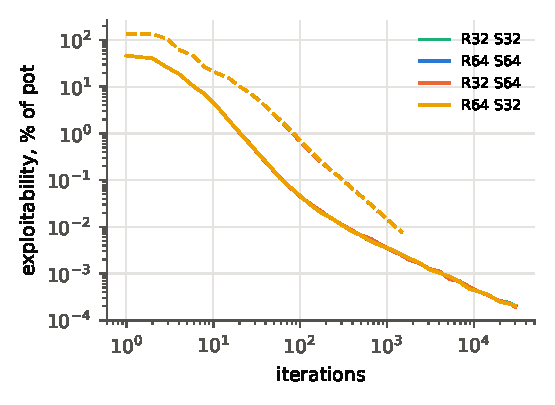
\includegraphics[width=0.55\linewidth]{precision.pdf}\end{center}
All four curves reach the same exploitability, down to $2\times10^{-4}\,\%$ of the pot, a thousand times below the
practical target. Storage precision does not limit accuracy.

\subsection{The subtle finding: conditioning}
The exploitabilities agree, but the \emph{strategies} of the float32 and float64 runs differ slightly (an average
difference of about 0.007 in probabilities). Is that rounding damage? A control experiment answers it: run double
precision twice, with the input ranges changed in the 7th decimal place. Those two runs differ just as much (0.012 and
0.0075). So the difference is not about storage. Any microscopic change sends DCFR to a slightly different
near-equilibrium.

\begin{intuition}
Picture a wide, flat valley floor. Every point on the floor has almost the same height (exploitability near zero),
but the points are far apart (different strategies). A ball rolled from slightly different places stops at different
spots on the floor. Numerical analysts say the strategy is \textbf{ill-conditioned} with respect to exploitability:
a tiny tolerance in the measure of quality allows a large range of answers. The solver guarantees the height, not the
spot.
\end{intuition}

\begin{example}[Ill-conditioning in a tiny linear system]
Solve $x+y=2$ and $x+1.0001y=2.0001$: the answer is $(1,1)$. Change the last number to $2.0002$: the answer becomes
$(0,2)$. A change in the 5th digit of the data moved the answer by 1. Both answers nearly satisfy both original
equations. That is ill-conditioning: small residual, large uncertainty in the solution.
\end{example}

\begin{takeaway}
Single precision is enough: same exploitability at half the memory. Strategies near equilibrium are not unique to
many digits, and that is a property of the problem, not of rounding. To show it, we ran a control experiment.
\end{takeaway}

% ============================================================================
\section{Parallel computing: splitting by the first card}\slide{15}
\subsection{The idea}
After the first betting round a card is dealt. What happens after the 5\SP{} is independent of what happens after
the 9\HE: they are separate branches. So different processor cores (\emph{workers}) can handle different cards at
the same time. One \emph{coordinator} keeps the small top of the tree.

One traversal becomes three steps:
\begin{enumerate}[nosep]
\item The coordinator walks the top and records the reach vectors arriving at each ``deal a card'' node.
\item Each worker receives those vectors, computes the values under its own cards and returns their sum.
\item The coordinator adds the sums, divides by $K$ and finishes the top.
\end{enumerate}
Only short vectors travel between coordinator and workers (at most 44 kB per traversal), while each card's subtree
is millions of operations. Little communication, lots of independent work: the ideal situation for parallelism.

\subsection{A model for the speedup}
If the coordinator needs time $t_c$ and one card's subtree needs $t_1$, then with $P$ workers the busiest worker has
$\lceil K/P\rceil$ cards ($\lceil\cdot\rceil$ means round up) and
\[ T(P)\approx t_c+\lceil K/P\rceil\,t_1. \]
\begin{example}[The flop numbers]
There are $K=49$ possible turn cards. With one worker an iteration takes 2327 ms, so $t_1\approx2327/49=47.5$ ms
($t_c$ is under a millisecond). With two workers the busier one has $\lceil49/2\rceil=25$ cards:
$25\times47.5\approx1187$ ms predicted, 1212 ms measured. Speedup: $2317/1212=1.9$ on two cores.
With eight workers the model predicts $\lceil49/8\rceil=7$ cards, about 333 ms; this is an extrapolation, since the
test machine has two cores.
\end{example}
\begin{center}\begin{tabular}{lrrrrr}
\toprule
spot & seq. & $P=1$ & $P=2$ & model & speedup \\ \midrule
turn & 62 & 65 & 35 & 33 & 1.8 \\
flop & 2317 & 2327 & 1212 & 1187 & 1.9 \\
\bottomrule
\end{tabular}
\end{center}

\textbf{Same answer?} Almost. The only difference from the one-core solver is the \emph{order} in which the card
sums are added, and floating-point addition depends very slightly on order. The results agree to about 14 digits,
not bit for bit. That is expected and the slide says so.

\begin{takeaway}
The tree splits naturally at the first dealt card. Speedup is limited by the busiest worker's share of cards.
Measured: 1.9 times faster on 2 cores.
\end{takeaway}

% ============================================================================
\section{Convergence: how many iterations?}\label{sec:conv}\slide{16--17}
\subsection{Reading a log--log plot}
The convergence plots show exploitability against iterations with both axes logarithmic. On such a plot a power law
$\text{error}\approx C/T^{k}$ is a straight line with slope $-k$:
\begin{itemize}[nosep]
\item slope $-\tfrac12$: 100 times more iterations for 10 times less error (the theorem's worst case);
\item slope $-1$: 10 times more iterations for 10 times less error;
\item slope $-2$: 10 times more iterations for 100 times less error.
\end{itemize}
\begin{center}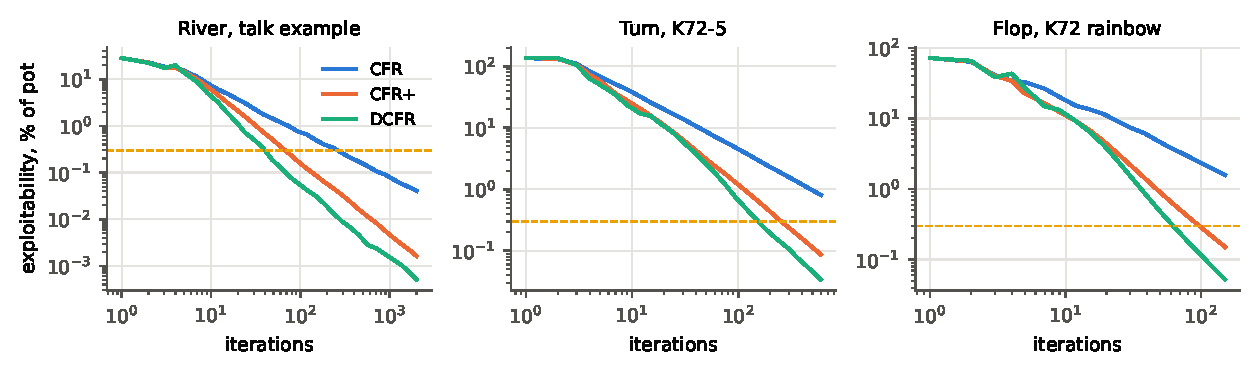
\includegraphics[width=\linewidth]{conv_streets.pdf}\end{center}
Measured slopes at the end of the runs: about $-1$ for CFR, $-1.4$ to $-1.7$ for CFR$^+$, and $-1.4$ to $-2.1$ for
DCFR. All are far better than the proven $-\tfrac12$. Nobody has a theory for why; that is an open research question.

\begin{example}[What the difference means]
After 150 iterations on the flop: CFR is at 1.6\% of the pot, CFR$^+$ at 0.15\%, DCFR at 0.05\%. Only DCFR is below
the 0.3\% target by a wide margin, after the same amount of work.
\end{example}

\textbf{Caution.} These slopes are measured over a limited window and depend on the window. They are observations,
not asymptotic rates. The slide words this carefully, and you should too.

\subsection{Iterations to a fixed accuracy}
The practical question is ``how many iterations until 0.3\%?'' Measured on 13 spots (median, with the range in
brackets):
\begin{center}\textit{pending}
\end{center}
So ``a few hundred iterations or fewer'' on every street. The count depends on the betting structure (how many bet
sizes and raises), not on the number of nodes:
\begin{center}\begin{tabular}{lrrr}
\toprule
K72 tree & decisions & 0.3\% & 0.1\% \\ \midrule
later streets checked down & 8 & 40 & 71 \\
river checked down & 789 & 40 & 71 \\
one size per street & 56,842 & 71 & 110 \\
standard & 85,263 & 110 & 196 \\
\bottomrule
\end{tabular}
\end{center}
The first two trees differ by a factor of 100 in size and need the same 40 iterations.

\begin{takeaway}
Total time = (iterations) $\times$ (time per iteration). The number of iterations is roughly the same everywhere, so
the \emph{cost per iteration} decides the running time. That is why most of the talk is about making one iteration
cheap.
\end{takeaway}

% ============================================================================
\section{Validation: how do we know it is right?}\slide{18}
A fast program that computes the wrong thing is worthless. Each part of the solver is checked against something
independent.

\textbf{Linear programming (LP) checks.} Small zero-sum games can be solved \emph{exactly} by a completely different
method, linear programming. We built small games a second time, in a different language (Python), with a different
representation, solved them by LP and compared the game value with DCFR's:
\begin{center}\begin{tabular}{lll}
\toprule game & DCFR value & LP value\\ \midrule
turn, 14 and 12 hands & 24.92419862 & 24.92419856\\
flop, 6 and 5 hands & 27.139343 & 27.139333\\
turn, 40 and 35 hands & 2.26976132 & 2.26976132\\ \bottomrule
\end{tabular}\end{center}
Agreement to 6 to 9 digits. The tiny differences are smaller than the exploitability left in the DCFR run, as they
should be.

\textbf{Why compare values and not strategies?} Because of the flat valley of Section 11: many different strategies
are equally good, but the \emph{value} of the game is unique.

\textbf{Other checks.} Fast leaves against the slow double loop (12 digits). Parallel against one-core (14 digits).
The zero-reach shortcut against no shortcut (bit for bit). The preflop solver against an LP (5 digits).

\textbf{What is not checked.} The flop solver has not yet been compared with an established solver on a full-size
tree. The talk says this on the Limitations slide, and it is the first item of Next steps.

\begin{takeaway}
Validate each component against an independent method, compare quantities that are unique, and say plainly what has
not been validated.
\end{takeaway}

% ============================================================================
\section{Extensions built on the same core}
\subsection{Node locking}\slide{20}
\emph{Locking} fixes one player's strategy at one decision point and re-solves everything else. It answers: ``my
opponent makes this specific mistake; how should I adjust?'' Technically, the locked node's regrets are frozen and
the solver finds the equilibrium of the \emph{restricted game}.

\begin{example}
On a river spot, the button in equilibrium never bets a third of the pot after a check. Lock him to always make that
bet. The big blind then folds 29\% instead of 49\%, and her value improves from $-16.2$ to $-6.2$ chips per hand:
betting every hand is a costly mistake. The locked game took 27 iterations to reach 0.3\%, the free game 40, so
locking is no harder to solve.
\end{example}
A subtlety from the slide: the 49\% is the response to a bet that never happens in equilibrium. Game theory does not
pin down what to do in situations that never occur, so that number is one valid answer among many.

\subsection{Aggregate flop reports}\slide{21}
A report solves the same spot on many flops and averages, to answer questions like ``how often should the big blind
bet across all flops?'' There are $\binom{52}{3}=22{,}100$ flops, but suits are interchangeable, so many flops are
strategically the same.

\begin{example}[Counting the truly different flops]
\emph{Three different ranks} ($\binom{13}{3}=286$ choices): the suits can be all different (``rainbow''), two alike
(three ways to choose which two ranks share a suit), or all alike (``monotone''). That is 5 patterns:
$286\times5=1430$.

\emph{A pair plus another card} ($13\times12=156$ choices): the third card either shares a suit with one of the pair
or not. 2 patterns: $156\times2=312$.

\emph{Three of a kind}: 13.

Total: $1430+312+13=1755$, the number on the slide. Each pattern stands for 24, 12 or 4 actual flops; for instance a
rainbow flop has $4\cdot3\cdot2=24$ suit assignments. (The slide derives the same number with group theory, the
symmetric group $S_4$ acting on suits, and Burnside's lemma.)
\end{example}

Solving 1755 flops is slow, so we solve a sample and weight each flop by how many flops it stands for. The sample is
\emph{stratified}: flops are grouped by type and each group is sampled in proportion, which is more accurate than
sampling at random. The $\pm$ in the table is a \emph{standard error}, the typical size of the sampling error:
\begin{center}\begin{tabular}{rrrr}
\toprule
flops & big blind value & solver bound & big blind bets \\ \midrule
25 & -0.450 $\pm$ 0.018 & 0.0047 & 19.8 $\pm$ 0.9\% \\
49 & -0.436 $\pm$ 0.019 & 0.0048 & 21.0 $\pm$ 1.0\% \\
95 & -0.453 $\pm$ 0.012 & 0.0048 & 20.9 $\pm$ 0.6\% \\
\bottomrule
\end{tabular}
\end{center}
With 25, 49 or 95 flops the answers agree within their error bars. The ``solver bound'' column is the error from not
solving each flop exactly (at most twice the exploitability); it is smaller than the sampling error, so sampling is
the limiting factor.

\subsection{Preflop and card removal between classes}\slide{22}
Before the flop, hands are grouped into 169 \emph{classes}: 13 pairs (6 combinations each), 78 suited hands (4
each) and 78 offsuit hands (12 each); indeed $13\cdot6+78\cdot4+78\cdot12=1326$. The preflop solver works with
vectors of length 169. It ends every hand that sees a flop with an all-in showdown, so later betting is not modelled
(a stated limitation).

Card removal now acts between classes: the matrix entry $M_{ij}$ is the fraction of (combination of $i$, combination
of $j$) pairs that can coexist.
\begin{example}[Three entries of $M$]
\textbf{AA against 72 offsuit:} no shared ranks, every pair is possible, $M=1$.

\textbf{AA against AK suited:} AA has 6 combinations, AKs has 4, so 24 pairs. For A\SP K\SP, the AA combinations
without the A\SP{} number $\binom32=3$. So $4\times3=12$ pairs are possible and $M=12/24=0.5$. Holding AK makes it
half as likely that the opponent has aces.

\textbf{AA against AA:} if I hold two aces, exactly one of the 6 combinations remains. $M=6/36=1/6$.
\end{example}
$M$ equals 1 except for classes that share a rank (27\% of entries), so multiplying by $M$ is ``sum everything,
then fix a few entries'', the same structural trick as in Section~\ref{sec:leaves}.

The simplest preflop game, \emph{push or fold} (all-in or fold), checks the solver against an LP:
\begin{center}\begin{tabular}{rrrrr}
\toprule
stack & LP value & DCFR value & push & call \\ \midrule
5 bb & 0.05616 & 0.05616 & 71.5\% & 62.0\% \\
10 bb & -0.04538 & -0.04538 & 58.2\% & 37.3\% \\
15 bb & -0.12721 & -0.12721 & 45.2\% & 28.5\% \\
20 bb & -0.18316 & -0.18316 & 40.2\% & 21.8\% \\
\bottomrule
\end{tabular}
\end{center}
With 10 big blinds the small blind goes all-in with 58\% of hands and the big blind calls with 37\%, matching
published charts.

\subsection{Errors in the data: a perturbation lemma}\slide{23}
The preflop solver uses a table of ``how often does class $i$ beat class $j$'', estimated by dealing random boards
(a \emph{Monte Carlo} estimate). The table has small random errors. So we are solving a slightly wrong game. How
wrong is the answer?

\textbf{Lemma.} If every payoff of a game is changed by at most $\delta$, then a strategy pair that is within
$\varepsilon$ of equilibrium in the changed game is within $\varepsilon+\delta$ in the original.

\begin{intuition}
If every outcome is mismeasured by at most one cent, no strategy's average outcome is off by more than one cent,
so nobody's best deviation gains more than about a cent beyond what we thought.
\end{intuition}
This is the game-theory version of a central question in numerical analysis: \emph{how do errors in the input
propagate to the output?} The lemma gives a worst case. The experiment (two independent tables, solve with one, test
in the other) shows the actual effect is 10{,}000 to 100{,}000 times smaller than the worst case, because random
errors of opposite signs cancel when averaged over a range.

\subsection{Three players at showdown: low-rank approximation}\slide{24}
With three players all-in we need the chance that class $i$ beats classes $j$ and $k$ together: a table $F$ with
$169^3\approx4.8$ million entries, used in a triple sum that is too slow.

For each $i$, the slice $F_i$ is a symmetric $169\times169$ matrix. Any symmetric matrix can be written as a sum of
simple ``rank-one'' pieces $\lambda\,uu^\top$ (its eigen-decomposition). Keeping only the 16 most important pieces
gives an approximation that is about five times cheaper to use:
$169^2/(2\cdot169\cdot16)\approx5.3$.

\begin{example}[A rank-one matrix]
$u=(1,2,3)$ gives $uu^\top=\begin{pmatrix}1&2&3\\2&4&6\\3&6&9\end{pmatrix}$. Nine entries, but only three numbers of
information. To compute $a^\top(uu^\top)b$ you do not need the nine entries: it equals $(u\cdot a)(u\cdot b)$, two dot
products. Low-rank approximation replaces a big table by a few such pieces.
\end{example}
The measured error of the quantity we actually need is 0.3\% at rank 16.

\subsection{More than two players}\slide{25}
With three or more players the theory breaks: there is no minimax theorem and DCFR is not guaranteed to converge.
We run it anyway and \emph{measure} the result with \textbf{NashConv}, the total amount all players together could
gain by deviating. Push-or-fold games get to about $10^{-6}$ big blinds (essentially exact). A realistic six-player
game stalls near 0.06 big blinds: decent, but not an equilibrium.

% ============================================================================
\section{Limitations and next steps}\slide{26--27}
A good talk says what is not done. Ours lists: the browser solver is slow compared with commercial ones (seconds per
flop iteration); the fast convergence has no theory; the preflop model ignores later betting; multiway has no
guarantee; parallel speedup was measured on two cores only; and the flop solver has not been compared against an
established solver on a full tree.

Next steps: that comparison first; then the high-precision ``Newton finish'' from the earlier talk; using suit
symmetry to solve fewer cards; faster compiled code; and pruning that keeps the iterations exact (remember the bug
story of Section 5).

% ============================================================================
\section{Glossary}
\begin{description}[leftmargin=1.2em,itemsep=1pt]
\item[Best response] The best possible strategy against a fixed opponent strategy.
\item[CFR] Counterfactual regret minimization: regret matching at every decision point of a game tree.
\item[Chance node] A point in the tree where a card is dealt.
\item[Conditioning] How much the answer can change when the data or tolerance changes a little.
\item[Counterfactual value] Value of an action weighted by the opponent's (and the cards') probability of reaching the point.
\item[DCFR] CFR with discounting of old regrets and old strategies.
\item[Exploitability] Average gain available to the players by best-responding; the solver's error measure.
\item[Hold-out validation] Testing a fitted model on data not used in the fit.
\item[Information set] A decision point as seen by a player holding a particular hand.
\item[Iteration] One update of both players' regrets and strategies (two tree traversals).
\item[Leaf] End of the hand in the tree: a fold or a showdown.
\item[Linear program (LP)] An optimization problem with linear objective and constraints; solves small zero-sum games exactly.
\item[Node locking] Fixing a strategy at one node and re-solving the rest.
\item[$O(n)$, $O(n^2)$] Work proportional to $n$, or to $n^2$, for large $n$.
\item[Public tree] The game tree of public events only; private hands live in vectors.
\item[Range] A vector of weights over a player's possible hands.
\item[Reach] The probability that a player's strategy brings a given hand to a given node.
\item[Regret] How much better an action would have done than what was played.
\item[Single/double precision] Number formats with about 7 and 16 significant digits.
\item[Standard error] The typical size of the error of an estimate from a sample.
\end{description}

\section{Check yourself}
\begin{enumerate}[itemsep=2pt]
\item Why does a solver output probabilities instead of one best action per hand?
\item In the toy game, what is the exploitability if the caller always \emph{calls} and the bettor plays the
equilibrium?
\item Cumulative regrets are $(3,-2,1)$. What does regret matching play next?
\item I hold Q\SP J\SP. The opponent's total weight is 10, his hands with the Q\SP{} weigh 1.5, with the J\SP{}
weigh 2, and Q\SP J\SP{} itself weighs 0.5. What is the compatible weight?
\item Why is $K=44$ on the turn?
\item A method's error falls from $10^{-2}$ to $10^{-4}$ when iterations go from 100 to 1000. What is the slope on a
log--log plot?
\item With 49 cards and 4 workers, how many cards does the busiest worker get?
\item Why compare game values, not strategies, when validating?
\end{enumerate}
\textbf{Answers.} (1) A predictable player can be exploited; equilibrium requires mixing. (2) The bettor's best
reply is to stop bluffing: value $\tfrac12\cdot2=1$ against $\tfrac12\cdot2+\tfrac12\cdot\tfrac12\cdot(-1)=0.75$ for
the equilibrium mix, gain 0.25, so again 12.5\% of the pot. (3) $(\tfrac34,0,\tfrac14)$. (4) $10-1.5-2+0.5=7$.
(5) $52-4$ board cards $-4$ private cards. (6) $-2$. (7) $\lceil49/4\rceil=13$. (8) Near-equilibrium strategies are
not unique, the value is.
\end{document}
